%======   Template created by Jonathan Blair  ========
%=====================================================

%=====================================================
%============ Controls ===============================
%=====================================================

%\documentclass[12pt,letterpaper,onecolumn]{article}
%\documentclass[11pt,letterpaper,onecolumn]{article}
%\documentclass[10pt,letterpaper,onecolumn]{article}
\documentclass[12pt,letterpaper,twocolumn]{article}
%\documentclass[11pt,letterpaper,twocolumn]{article}
%\documentclass[10pt,letterpaper,twocolumn]{article}


\usepackage{amsmath}
\usepackage{graphics}
\usepackage{graphicx} %more modern version of graphics
\usepackage{caption}
\usepackage[section]{placeins}
\usepackage{float}
%\graphicspath{{path-to-folder-containing-necessary-graphics}{other folder as necessary}}


%=====================================================
%============ \begin{document} =======================
%=====================================================

\begin{document}

%=====================================================
%============ Title ==================================
%=====================================================

\title{Investigating Temperature and Voltage Dependence in NPN Bipolar Junction Transistors}
%\title{\Large\bf Larger, Bolded Title}

%=====================================================
%============ Author =================================
%=====================================================
\author{
 Garik Livingston and Lily Nguyen \\*
  \\*
 PHY 353L Modern Laboratory \\*
 Department of Physics \\*
 The University of Texas at Austin \\*
 Austin, TX 78712, USA
}
\date{February 11, 2025}

%\address{The University of Texas, Austin, Texas, 78712}

\maketitle

%=====================================================
%============ Abstract ===============================
%=====================================================

\begin{abstract}
	In this experiment, we varied the voltage supplied to the base of a NPN BJT transistor and measured the current running through the collector to form a data set which we fitted to the Ebbers-Moll equation.
	From this fit we calculated the thermal voltage ($V_T$) and saturation current ($I_s$). Both these paramaters have strong temperature dependence and from our fit we determined an experimental value for the boltzman constant of $k = 1.389 \times 10^{-23} \pm 2.19 \times 10^{-26} \frac{J}{K}$ for the silicon transistor and a value of k = $5.617 \times 10^{-23}\pm 8.99 \times 10^{-26} \frac{J}{K}$ for the germanium transistor. 
	We also determined an experimental value for the band gap of the transistors with a $E_g = 1.48 \pm 0.012eV$ for silicon and  $E_g = 0.158 \pm 0.003 eV$ for germanium.
	
\end{abstract}

%=====================================================
%============ Body of the article ====================
%=====================================================

%=====================================================
%============ Section ================================

\section{Introduction}

\subsection{Physics Motivation}

Semiconductors are essential components of modern electronics due to their unique electronic properties: a valence band filled with electrons and a nearly empty conduction band, separated by an energy band gap \( V_g \). The ability of electrons to transition from the valence band to the conduction band under specific conditions, such as thermal excitation or applied voltage, forms the basis for the functionality of semiconductor devices like transistors \cite{Thornton}.

%<<<<<<< HEAD
In this experiment, we explore the behavior of an NPN bipolar junction transistor (BJT) and focus on the relationship between the collector current \( I_C \) and the base emitter voltage \( V_{BE} \). The function of the transistor depends on the exponential dependence of \( I_C \) on \( V_{BE} \), described by the Ebers-Moll equation.

%=======
In this experiment, we investigate the behavior of an NPN bipolar junction transistor (BJT) by examining the relationship between the collector current \( I_C \) and the base-emitter voltage \( V_{BE} \). The transistor’s function depends on the exponential dependence of \( I_C \) on \( V_{BE} \), described by the Ebers-Moll equation:
\begin{equation}\label{eq1}
%>>>>>>> a9e140ca79745e5e2c7135285a616d71aedfce01
I_C = I_S \left(e^{eV_{BE}/kT} - 1\right)
\end{equation}

where \( I_S \) is the saturation current, \( e \) is the elementary charge, \( k \) is the Boltzmann constant and \( T \) is the absolute temperature \cite{Neudeck}. This exponential behavior arises from the Boltzmann factor, which governs the probability of electron excitation across the band gap:

\begin{equation}\label{eq2}
P(E) \propto e^{-E/kT}
\end{equation}

By measuring \( I_C \) as a function of \( V_{BE} \) at different temperatures, we can extract both Boltzmann’s constant and the band gap of the semiconductor material. This experiment not only reinforces the theoretical principles of semiconductor physics, but also demonstrates the practical application of transistors in amplification and switching, which are fundamental to all modern electronic devices \cite{Thornton}.


\subsection{Historical context}

The invention of the bipolar junction transistor (BJT) in 1947 by John Bardeen, Walter Brattain, and William Shockley marked a pivotal moment in semiconductor technology. Their initial device, the germanium point-contact transistor, exhibited power gain but was unstable and difficult to reproduce due to sensitivity to surface states and impurities \cite{Lukasiak}. Shockley later developed the p-n junction transistor, which proved more reliable by utilizing bulk conduction of minority carriers. This advancement earned the trio the Nobel Prize in Physics in 1956.

Early transistors were difficult to manufacture consistently. The development of grown junction transistors in 1952 improved stability, but the process remained complex and wasteful. The introduction of the alloyed junction transistor in the same year simplified production and reduced material waste. By 1954, diffused junction transistors allowed for more precise control over transistor properties, enabling higher-frequency operation. The shift from germanium to silicon further improved the performance as a result of the lower reverse currents of silicon and better thermal stability. The first commercial silicon transistors were produced by Gordon Teal in 1954, with planar transistors introduced by Jean Hoerni in 1960, enabling mass production and miniaturization \cite{Lukasiak}.

These advancements laid the foundation for modern experimental techniques. Early measurements were manual and prone to errors, while today's experiments leverage automated voltage sweeps with precise current measurements. Controlled temperature environments using thermocouples and heating setups allow for detailed analysis of the temperature dependence of the collector current \( I_C \). These techniques facilitate the verification of theoretical models such as the Ebers-Moll equation and the determination of constants such as the Boltzmann constant and the semiconductor band gap.


%=====================================================
%============ Section ================================

\section{Theoretical background}

Semiconductors are materials characterized by an electronic structure consisting of a valence band filled with electrons and a conduction band that is nearly empty at low temperatures. These bands are separated by an energy gap, known as the band gap \( V_g \). At absolute zero, semiconductors behave as insulators, with no electrons in the conduction band. However, at finite temperatures, some electrons gain enough thermal energy to cross the band gap, enabling electrical conduction. The likelihood of electron excitation across the band gap is determined by the Boltzmann factor:

\begin{equation}\label{eq3}
P(E) \propto e^{-E/kT}
\end{equation}

where \( E \) is the energy required for excitation, \( k \) is Boltzmann’s constant, and \( T \) is the absolute temperature\cite{Thornton}.

An NPN bipolar junction transistor (BJT) consists of two n-doped regions (the emitter and collector) separated by a thin p-doped base. When a positive voltage is applied to the base relative to the emitter (\( V_{BE} \)), it reduces the potential barrier, allowing electrons from the emitter to be injected into the base. Due to the thinness of the base and the applied positive voltage at the collector, most of these electrons drift into the collector, resulting in a measurable collector current \( I_C \) \cite{Neudeck}.

The relationship between the collector current \( I_C \) and the base-emitter voltage \( V_{BE} \) is described by the Ebers-Moll equation:

\begin{equation}\label{eq4}
I_C = I_S \left(e^{\frac{eV_{BE}}{kT}} - 1\right)
\end{equation}

where \( I_S \) is the saturation current, \( e \) is the elementary charge, \( k \) is Boltzmann’s constant, and \( T \) is the absolute temperature. This equation illustrates the exponential dependence of \( I_C \) on \( V_{BE} \), a fundamental property that allows transistors to function as amplifiers and switches in electronic circuits\cite{Neudeck}.

The saturation current \( I_S \) itself is temperature-dependent and follows the relation:

\begin{equation}\labe{eq5}
I_S \propto e^{-V_g/kT}
\end{equation}

This indicates that \( I_S \) increases exponentially with temperature as more electrons acquire sufficient energy to cross the band gap \( V_g \). By plotting \( \ln(I_S) \) against \( 1/T \), the band gap of the semiconductor can be extracted from the slope of the linear fit:

\begin{equation}\label{eq6}
\ln(I_S) = -\frac{V_g}{kT} + \text{constant}
\end{equation}

Additionally, analyzing the exponential dependence of \( I_C \) on \( V_{BE} \) at various temperatures allows for the determination of Boltzmann’s constant. The thermal voltage \( V_T \), defined as:

\begin{equation}\label{eq7}
V_T = \frac{kT}{e}
\end{equation}


also plays a crucial role in the transistor’s behavior, influencing the rate at which \( I_C \) increases with \( V_{BE} \)\cite{Collings1980}.

In this experiment, we measure \( I_C \) as a function of \( V_{BE} \) at different temperatures to extract both Boltzmann’s constant and the semiconductor band gap. These measurements validate theoretical models and provide insight into the intrinsic properties of semiconductor materials like silicon and germanium.


%=====================================================
%============ Section ================================

\section{Experimental setup}


\subsection{Apparatus}

This experiment investigates the temperature and voltage dependence of an NPN Bipolar Junction Transistor (BJT) by analyzing the relationship between the base-emitter voltage (\( V_{BE} \)) and the resulting collector current (\( I_C \)). The goal is to study the exponential behavior of \( I_C \) as described by the Ebers-Moll equation and to extract key physical constants such as Boltzmann’s constant and the semiconductor band gap \cite{Neudeck}.

The transistor is mounted on an aluminum plate to enable controlled temperature variation. Heating is provided using a GwINSTEK GPS-3030DD Laboratory DC Power Supply connected to a 25 W power resistor clamped to the plate. A Type K thermocouple, integrated with the Omega HH12C Temperature Probe, measures the transistor’s temperature with high precision, as precise thermal management is essential for accurate semiconductor characterization \cite{Grundmann}. For cryogenic measurements, the transistor is submerged in liquid nitrogen to investigate low-temperature behavior.

A programmable voltage source, controlled via LabView’s \texttt{semiconductor.vi} and interfaced through a Texas Instruments NI USB-6341 X Series Multifunction DAQ, applies precise voltages to the base-emitter junction. The DAQ ensures synchronized voltage control and current measurements, enabling automated data collection. The collector current (\( I_C \)) is measured using a Keithley 6485 Picoammeter, which offers high sensitivity across several orders of magnitude, from nanoamps to milliamps. A 1 k\(\Omega\) resistor is placed in series with the collector to limit current and protect the transistor.

Connections between the transistor, power supply, and measurement instruments are established using BNC banana plugs, BNC female adapters, and coaxial cables to minimize electrical noise. Simple wires and a short wire are used to complete the circuit and ensure stable connections throughout the setup.

The experimental procedure is also repeated with a germanium transistor to compare its temperature-dependent behavior with that of silicon, enabling validation of extracted values for Boltzmann’s constant and the band gap \cite{Collings}.

\begin{figure}[H]
\centering
\includegraphics[width=0.5\textwidth]{experimental_setup.png}
\caption{Schematic of the experimental setup, including the NPN BJT transistor, Keithley Picoammeter, DC power supply, and temperature control system.}
\label{fig:apparatus}
\end{figure}


%=====================================================
%============ Importing pictures  ====================
%=====================================================

\subsection{Data Collection}
We setup our circuit to have a variable supply of voltage to the base ($V_{be}$) while measuring the collector current ($I_c$) readings from the pico ampmeter.
We then supplied voltage to the thermocouple and watied for the temperature of the transistor to reasonbly level out before we recorded a $I_c \text{ vs } V_{be}$ data set.


%Data taking procedures should be described and various modes of
%data collection explained. Calibration procedures and
%relevant plots and numerical tables should be included.
%State clearly what measurements were taken for the final
%data analysis. Describe `doing the experiment' so it would
%be helpful to other students in the future. This may need
%to include physics arguments {\em what } and {\em how } data should
%be collected.


\subsection{Data Analysis}
\subsubsection{$V_T \text{ vs } T$}
We took the dataset of $I_c \text{ vs }V_{be}$ and fitted it to \ref{eq4}. We determined an experimental value and standard error for $V_T$ using the curve fit function from scipy.

\begin {table}[H]
\caption*{Silicon Data}
{\footnotesize
\begin {center}
\begin {tabular} {|c | c | c| }
\hline
Temps (K) 			&    $V_T$		& Err($V_T$)\\
\hline  &&\\
296.4   & 0.0247 &  0.000137\\
\hline  && \\
297.4   & 0.02554 &  3.54e-05\\
\hline  && \\
298.8   & 0.02568 &  2.763e-05\\
\hline  && \\
300.1   & 0.02579 &  3.376e-05\\
\hline  && \\
302.0   & 0.02599 &  3.060e-05\\
\hline  && \\
306.1   & 0.02644 &  2.216e-05\\
\hline  && \\
307.5   & 0.02659 &  2.194e-05\\
\hline  && \\
313.3   & 0.02718 &  1.825e-05\\
\hline  && \\
316.1	& 0.02746 &  1.864e-05\\
\hline% \hline
\end {tabular}
\end {center}
}
\caption{\label{tab1} $V_T \text{ vs } T$ data for silicon transistor}
\end {table}

\begin {table}[H]
\caption*{Germanium Data}
{\footnotesize
\begin {center}
\begin {tabular} {|c | c | c| }
\hline
Temps (K) 			&    $V_T$		& Err($V_T$)\\
\hline&&\\
296.4 & 0.104 & 0.00211\\
\hline  && \\
296.6 & 0.104 & 0.00211\\
\hline  && \\
297.4 & 0.104 & 0.00209\\
\hline  && \\
298.5 & 0.105 & 0.00215\\
\hline  && \\
300.0 & 0.105 & 0.00210\\
\hline  && \\
301.7 & 0.106 & 0.00221\\
\hline  && \\
302.1 & 0.106 & 0.00215\\
\hline  && \\
305.5 & 0.107 & 0.00222 \\
\hline  && \\
307.1 & 0.107 & 0.00213 \\
\hline  && \\
308.1 & 0.109 & 0.00228\\
\hline  && \\
312.6 & 0.109 & 0.00230\\
\hline  && \\
315.2 & 0.110 & 0.00236\\
\hline% \hline
\end {tabular}
\end {center}
}
\caption{\label{tab2} $V_T \text{ vs } T$ data for germanium transistor}
\end {table}

We then performed a weighted least square analysis with \ref{eq7} as the model, and with the variance of $V_T$ found from curve fit. We expected the slope to equal $\frac{k}{e}$. We performed this analysis for both the silicon and germanium transistor data. 

\begin{figure}[H]
	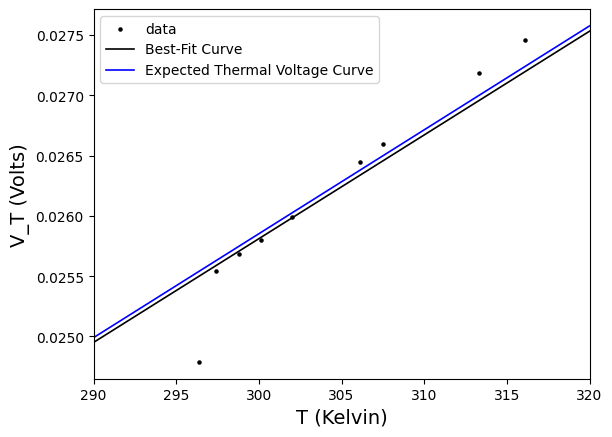
\includegraphics[width = .5\textwidth]{2_6SiBoltz.png}
	\caption{Silicon temperature vs thermal voltage graph. The data points collected are represented by the black dots, our best-fit slope is the solid black curve, and the expected slope of $\frac{k}{e}$ is the solid blue curve.\label{g1}}
\end{figure}
\begin{figure}[H]
	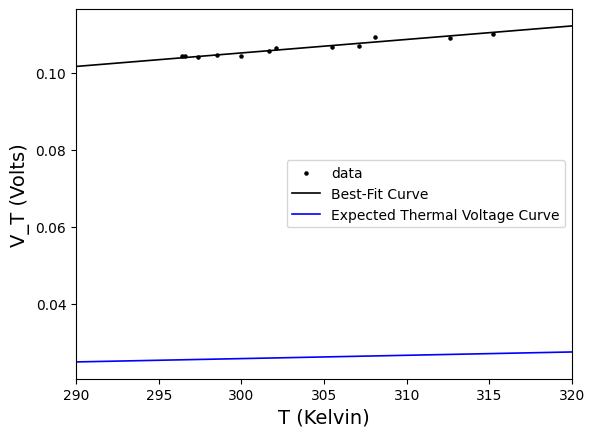
\includegraphics[width = .5\textwidth]{GeBoltz.png}
	\caption{Germanium temperature vs thermal voltage graph. The data points collected are represented by the black dots, our best-fit slope is the solid black curve, and the expected slope of $\frac{k}{e}$ is the solid blue curve.\label{g2}}
\end{figure}

\subsubsection{$I_s \text{ vs }T$}
We took the dataset of $I_c \text{ vs }V_{be}$ and fitted it to \ref{eq4}. We determined an experimental value and standard error for $I_s$ using the curve fit function from scipy.

\begin {table}[H]
\caption*{Silicon Data}
{\footnotesize
\begin {center}
\begin {tabular} {|c | c | c| }
\hline
Temps (K) 			&    $I_s$(Pico Amps) & Err($I_s$)\\
\hline  &&\\
296.4   & 0.24 & 0.0243\\
\hline  && \\
297.4   & 0.46 & 0.0121\\
\hline  & &\\
298.8   &0.59  & 0.0120\\
\hline  && \\
300.1   &0.73  &  0.0179\\
\hline  & &\\
302.0   &1.00  & 0.0220\\
\hline  & &\\
306.1   &2.09  &  0.0320\\
\hline  & &\\
307.5   &2.65  &  0.0397\\
\hline  & &\\
313.3   &6.84  &  0.0816\\
\hline  & &\\
316.1	&10.2  & 0.122\\
\hline% \hline
\end {tabular}
\end {center}
\caption{\label{tab1} $I_s \text{ vs } T$ data for silicon transistor}
}
\end{table}
\begin {table}[H]
\caption*{Germanium Data}
{\footnotesize
\begin {center}
\begin {tabular} {|c | c | c| }
\hline&&\\
Temps (K) 			&    $I_s$(Pico Amps) & Err($I_s$)\\
\hline&&\\
296.4 & 0.00013 & 1.015e-05\\
\hline &&\\                
296.6 & 0.00013 & 1.015e-05\\
\hline &&\\                
297.4 & 0.00013 & 1.018e-05\\
\hline &&\\                
298.5 & 0.00013 & 1.076e-05\\
\hline &&\\                
300.0 & 0.00014 & 1.074e-05\\
\hline &&\\                
301.7 & 0.00015 & 1.172e-05\\
\hline &&\\                
302.1 & 0.00015 & 1.162e-05\\
\hline &&\\                
305.5 & 0.00017 & 1.274e-05\\
\hline &&\\                
307.1 & 0.00017 & 1.261e-05\\
\hline &&\\                
308.1 & 0.00019 & 1.415e-05\\
\hline &&\\                
312.6 & 0.00020 & 1.523-05 \\
\hline &&\\                
315.2 & 0.00022 & 1.643e-05\\
\hline% \hline
\end {tabular}
\end {center}
\caption{\label{tab1} $I_s \text{ vs } T$ data for germanium transistor}
}
\end{table}

As our range of temperatures [296K,316K] was small, we performed a weighted least squares analysis with \ref{eq6} as the model, and the variance for $I_s$ derived from curve fit.

\begin{figure}[H]
	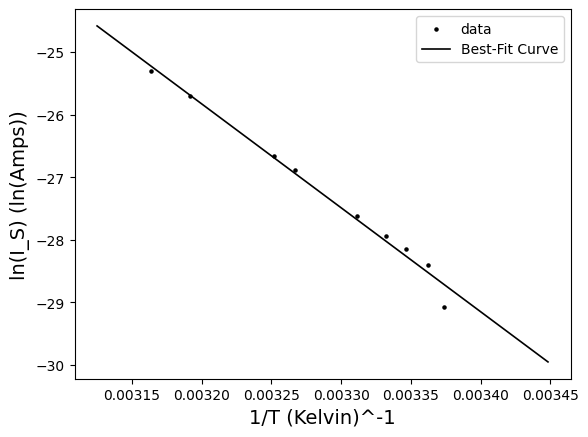
\includegraphics[width = .5\textwidth]{linSiSatCurrent.png}
	\caption{Silicon saturation current vs temperature. The data points collected are represented by the black dots, and our best-fit slope is the solid black curve.\label{g3}}
\end{figure}
\begin{figure}[H]
	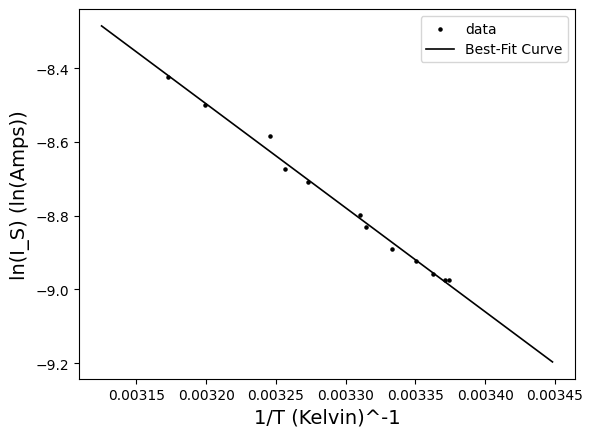
\includegraphics[width = .5\textwidth]{linGeSatCurrent.png}
	\caption{Germanium saturation current vs temperature. The data points collected are represented by the black dots, and our best-fit slope is the solid black curve.\label{g4}}
\end{figure}
We note there was much greater error in the germanium data than the silicon we theorize this is a combination of both the greater amount of "natural" distortion in germanium transistors, and perhaps a paricular fault with our germanium transistor.

\section{Results}
The slope of the best fit curve from figure 2 was found to be $8.67 \times 10^{-5} \pm 1.37 \times 10^{-7} \frac{J}{KC}$, and the slope of the best fit curve from figure 3 was found to be $3.506 \times 10^{-4} \pm 5.61\times 10^{-7}\frac{J}{KC}$. We expected to find a slope of $\frac{k}{e} = 8.617 \times 10^{-5}\frac{J}{KC}$. The slope of the best curve from figure 4 was found to be $-1.66 \times 10^{4} \pm 716.863 \frac{K}{C}$, and the slope of the best curve from figure 5 was $-2820 \pm 76.537 \frac{K}{C}$. We expected to find a slope of $\frac{-E_g}{k} = \frac{-1.1}{k} = -1.2769565 \times 10^{4} \frac{K}{C}$ for figure 4 and a slope of $\frac{-E_g}{k} = \frac{-0.7}{k} = -8126.087 \frac{K}{C}$ for figure 5.
In more familiar terms, from figure 2 we found an experimental value of $k = 1.389 \times 10^{-23} \pm 2.19 \times 10^{-26} \frac{J}{K}$, from figure 3 we found an experimental value of $k = 5.617\times 10^{-23} \pm 8.99 \times 10^{-26}\frac{J}{K}$. We also found an experimental value for the bandgap of a silicon transistor to be $1.43 \pm 0.0618 eV$ and $0.243 \pm 0.0066 eV$ for the germanium transistor. We expected a value of $k = 1.380 \times 10^{-23} \frac{J}{K}$ for the boltzman constant, a $E_g = 1.1eV$ for the silicon transistor, and $E_g = 0.7 eV$ for the germanium transistor.

%=====================================================
%============ Section ================================

\section{Summary and conlcusions}
	We were able to calculate an experimental value for the boltzman constant that was reasonably close to the expected value for the silicon transistor. However, the germanium transistor produced a value for boltzman constant that was much further off than the we expected. In addittion to measuring the boltzman constant we also found experimental values for the band gap of the silicon and germanium transistors. These values both varied largely from the expected values. Overall, our experimental methods allowed us to accurately calculate the boltzman constant by studying the effect temperature had on the current running through a silicon transistor, but measurement of other constants such as the band gap were not sucessful. In addittion, the germanium transistor produced unreliable data that was likely a fault of our particular transistor.

%=====================================================
%============ Bibliography  ==========================
%=====================================================

\begin{thebibliography}{9}

\bibitem{Collings1980} 
P. J. Collings, 
\textit{Simple measurement of the band gap in silicon and germanium}, 
American Journal of Physics, \textbf{48}(3), 197--199 (1980). 
\href{https://doi.org/10.1119/1.12172}

\bibitem{Grundmann2016} 
M. Grundmann, 
\textit{The Physics of Semiconductors: An Introduction Including Nanophysics and Applications}, 3rd ed., 
Springer Nature, 2016. 
\href{https://doi.org/10.1007/978-3-319-23880-7}{https

\bibitem{Lukasiak} 
L. Łukasiak and A. Jakubowski, 
"History of Semiconductors," 
\textit{Journal of Telecommunications and Information Technology}, vol. 1, pp. 3–9, 2023. 
Available: \url{https://doi.org/10.26636/jtit.2010.1.1015}

\bibitem{Neudeck} 
G. W. Neudeck, 
\textit{The Bipolar Junction Transistor}, 2nd ed., 
Addison-Wesley, 1989.

\bibitem{Thornton} 
S. T. Thornton and A. F. Rex, 
\textit{Modern Physics for Scientists and Engineers}, 3rd ed., 
Thomson, Brooks/Cole, 2006.

\end{thebibliography}

%=====================================================
%============ End ====================================
%=====================================================

\end{document}

%=====================================================
%============ End ====================================
%=====================================================
